\documentclass[letterpaper]{exam}
\printanswers
\usepackage{hyperref}
\usepackage[utf8x]{inputenc}
\usepackage[table]{xcolor}
\usepackage{listings}
\usepackage{mdframed}
\usepackage{lmodern}
\usepackage[left=0.25in, right=0.25in, top=0.75in, bottom=0.75in]{geometry}
\usepackage{graphicx}
\usepackage{amsmath,amssymb}
\usepackage{tikz}
\usepackage{pgfplots}
\usepackage{subfigure}
\usepackage{enumerate}
\usepackage{tcolorbox}
\usepackage{float}
\pagestyle{headandfoot}

\usepackage{cancel}
\usepackage{placeins}
\usepackage{multirow}
\usepackage{algorithm2e}
\pagecolor{black}
\color{white}
\hypersetup{%
  colorlinks=true,% hyperlinks will be black
  linkbordercolor=red,% hyperlink borders will be red
  pdfborderstyle={/S/U/W 1}% border style will be underline of width 1pt
}

\newcommand{\soln}{\\ \textbf{Solution}: }
\newcommand{\bkt}[1]{\left(#1\right)}
\lhead{MA5892: Numerical Methods and Scientific Computing}

\chead{End Semester}

\rhead{Rollnumber: EE18B067}

\begin{document}
\hrule
\vspace{3mm}
\noindent 
\vspace{3mm}
\noindent{{\sf Roll No:} EE18B067 \hfill  {\sf Name:Abhishek Sekar}}% put your ROLL NO AND NAME HERE

\noindent
{{\sf Date: \today }} %Date
\vspace{3mm}
\hrule
\begin{questions}
\question [3] An integral of the form $\mathlarger{\mathlarger{\int}}_0^1$ f(x) dx was computed by two students using trapezoidal rule with end point corrections involving only the first derivative. The first student reported the value as 0.8 using a grid spacing of h, while the second student reported the value as 0.75 using a grid spacing of $\frac{h}{2}$.A smart, lazy student from NMSC class enters their discussion and gives a better answer of the integral with a higher
order of accuracy by processing the information above. How did he do it? What was his answer? What is the order of accuracy of his answer?
\begin{solution}
\\
\textbf{Expression for Trapezoidal Rule with end point correction:}\\
An integral of the form $\mathlarger{\mathlarger{\int}}_a^b$ f(x) dx can be approximated using Trapezoidal Rule with end point correction using the first derivative as follows:
\begin{align}\label{1}
\mathlarger{\mathlarger{\int}}_a^b f(x) dx &= \frac{h}{2}\cdot\left(f(a) + f(b)\right) + h \cdot \left(\overset{N-1}{\underset{i=1}{\sum}} f(x_i)\right) - \frac{b_2}{2!}\cdot h^2 \cdot \left(f^{'}(b) - f^{'}(a)\right) + \mathcal{O}\left(h^4\right)
\end{align}
where h is the grid spacing and N is the corresponding number of panels, where $N = \frac{b-a}{h}$. $b_2$ is the second Bernoulli number and is equal to $\frac{1}{6}$.\\
$\mathcal{O}\left(h^4\right)$ is the error term and comes from $\frac{-b_4}{4!}\cdot h^4 \cdot \left(f^{'''}(b) - f^{'''}(a)\right)$ where $b_4$ is the fourth Bernoulli number and has a value of $\frac{-1}{30}$.\\
We see that the given problem has b = 1 and a = 0.\\
\textbf{First Student's approximation}\\
The first student approximates the integral using a grid spacing of h.\\ 
Thus, including the expression of the error term as well, the student approximates the integral using \ref{1} as,
\begin{align}\label{2}
\mathlarger{\mathlarger{\int}}_0^1 f(x) dx &\approx 0.8 =  \frac{h}{2}\cdot\left(f(0) + f(1)\right) + h \cdot \left(\overset{\frac{1}{h}-1}{\underset{i=1}{\sum}} f(x_i)\right) - \frac{1}{12}\cdot h^2 \cdot \left(f^{'}(1) - f^{'}(0)\right) \\ 
\text{Error} &\approx \frac{1}{720}\cdot h^4 \cdot \left(f^{'''}(1) - f^{'''}(0)\right)
\end{align}
\textbf{Second Student's approximation}\\
The second student approximates the same integral using a grid spacing of $\frac{h}{2}$ and should hence get an approximation closer to the actual answer.\\
Thus the approximation is,
\begin{align}\label{3}
\mathlarger{\mathlarger{\int}}_0^1 f(x) dx &\approx 0.75 =  \frac{h}{4}\cdot\left(f(0) + f(1)\right) + \frac{h}{2} \cdot \left(\overset{\frac{2}{h}-1}{\underset{i=1}{\sum}} f(x_i)\right) - \frac{1}{12}\cdot \frac{h^2}{4} \cdot \left(f^{'}(1) - f^{'}(0)\right) \\ 
\text{Error} &\approx \frac{1}{720}\cdot \frac{h^4}{16} \cdot \left(f^{'''}(1) - f^{'''}(0)\right)
\end{align}
\textbf{Lazy Student's approximation}\\
Let us place ourselves in the lazy student's shoes.\\
We have access to approximations using grid spacing h in \ref{2} and approximations using grid spacing $\frac{h}{2}$ in \ref{3}, how do we improve the accuracy?\\
This train of thought gives us an idea. Perhaps, we could try cancelling the error term using a linear combination of both the expressions resulting in a much higher order of accuracy.\\
Thus, we see that the error term in \ref{2} is 16 times as large as that in \ref{3}.\\
To \textit{cancel} the (leading) error terms, we simply need to do $16 \cdot $\ref{3} - \ref{2}.\\
Thus, this leads us to the approximation shown below.
\begin{align*}
    16\mathlarger{\mathlarger{\int}}_0^1 f(x) dx - \mathlarger{\mathlarger{\int}}_0^1 f(x) dx &\approx 16\cdot(0.75) - 0.8 = 11.2
\end{align*}
Or from this, we obtain that the approximate value of the integral using this approach is $\frac{11.2}{15}$  = 0.746666667.\\
Using this approach, we're essentially treating the first order end point corrections as if they were end point corrections using both the first and the third derivatives (the third derivatives get "cancelled") thereby increasing the accuracy.\\
The order of accuracy of this answer is $\mathcal{O}\left(h^6\right)$ as in a trapezoidal rule with the above end point correction.\\
Note: Much higher accuracy answers can be obtained by repeatedly employing the above strategy. However, as the student is lazy, he might not pursue it!
\end{solution}
\question [10]  Gaussian quadrature:
\begin{parts}
\part [4] Find the first three monic polynomials (i.e., till quadratic) on [0, 1] orthogonal with respect to the inner product
\begin{align*}
    \left< f,g \right> &= \mathlarger{\mathlarger{\int}}_0^1 \frac{x}{\sqrt{1-x^2}} f(x)g(x)dx
\end{align*}
\begin{solution}
\\
Following the notation used in the course, let us denote the $n^{th}$ degree monic polynomial by $q_n(x)$.\\
As is convention, we take the $0^{th}$ degree monic polynomial $q_0(x) = 1$.\\
\textbf{Finding the first degree monic polynomial}\\
The first degree monic polynomial $q_1(x)$ is of the form x+c for some constant c $\in \mathbb{R}$.\\
We're given that the monic polynomials are orthogonal with respect to the given inner product.\\
Thus, we have,
\begin{align*}
     \left< q_0,q_1 \right> &= \mathlarger{\mathlarger{\int}}_0^1 \frac{x}{\sqrt{1-x^2}} q_0(x)q_1(x)dx \\ 
     &\Rightarrow
     \mathlarger{\mathlarger{\int}}_0^1 \frac{x}{\sqrt{1-x^2}} 1\cdot(x+c)dx \\
     &\Rightarrow
     \mathlarger{\mathlarger{\int}}_0^1 \frac{x^2}{\sqrt{1-x^2}} dx + \mathlarger{\mathlarger{\int}}_0^1 \frac{cx}{\sqrt{1-x^2}} dx
     &\Rightarrow
     I_1 + c\cdot I_2
\end{align*}
where $I_1 = \mathlarger{\mathlarger{\int}}_0^1 \frac{x^2}{\sqrt{1-x^2}} dx $ and $I_2 = \mathlarger{\mathlarger{\int}}_0^1 \frac{x}{\sqrt{1-x^2}} dx$.\\
Let us try solving these two integrals.\\
To solve $I_1$, we make the substitution $x = \cos{(\theta)}$. Therefore, $dx = -\sin{(\theta)} d\theta$ and the limits go from $\frac{\pi}{2}$ to 0 for this variable change.\\
Doing this, we get,
\begin{align*}
    I_1 &= \mathlarger{\mathlarger{\int}}_0^1 \frac{x^2}{\sqrt{1-x^2}} dx\\
    &\Rightarrow
    \mathlarger{\mathlarger{\int}}_{\frac{\pi}{2}}^0 \frac{\cos{ ^2(\theta)}}{\sqrt{1-\cos{ ^2(\theta)}}} -\sin{(\theta)} d\theta \\
    &\Rightarrow
    \mathlarger{\mathlarger{\int}}_0^{\frac{\pi}{2}} \frac{\cos{ ^2(\theta)}}{\sin{(\theta)}} \sin{(\theta)} d\theta\\
    &\Rightarrow
    \mathlarger{\mathlarger{\int}}_0^{\frac{\pi}{2}} \cos{ ^2(\theta)} d\theta\\
    &\Rightarrow
    \mathlarger{\mathlarger{\int}}_0^{\frac{\pi}{2}} \left(\frac{1 + \cos{(2\theta)}}{2}\right) d\theta\\
    &\Rightarrow
    \frac{1}{2}\cdot \left[\theta + \frac{\sin{(2\theta)}}{2}\right]_{0}^{\frac{\pi}{2}}\\
    &\Rightarrow
    \frac{\pi}{4}
\end{align*}
Therefore, $I_1 = \frac{\pi}{4}$.\\
Let us compute the integral $I_2$. To solve $I_2$, we make the substitution $t = 1-x^2$, thus, $dt = -2x dx$ and the limits go from 1 to 0 for this variable change.\\
Doing this, we get,
\begin{align*}
    I_2 &= \mathlarger{\mathlarger{\int}}_0^1 \frac{x}{\sqrt{1-x^2}} dx\\
    &\Rightarrow
    \mathlarger{\mathlarger{\int}}_1^0 -\frac{1}{2}\cdot\frac{-2x}{\sqrt{1-x^2}} dx\\
    &\Rightarrow
    \mathlarger{\mathlarger{\int}}_0^1 \frac{1}{2}\cdot\frac{1}{\sqrt{t}} dt\\
    &\Rightarrow
    \frac{1}{2}\cdot \left[2t^{\frac{1}{2}}\right]_{0}^1\\
    &\Rightarrow
    1
\end{align*}
Thus, our original integral $I_1 + cI_2$ becomes $\frac{\pi}{4} + c$.\\
But as $q_0(x)$ and $q_1(x)$ are orthogonal with respect to this inner product, $\frac{\pi}{4} + c = 0$ or $c = -\frac{\pi}{4}$.\\
Thus, the first degree monic polynomial $q_1(x) = x - \frac{\pi}{4} $.\\
\textbf{Finding the second degree monic polynomial}\\
The second degree monic polynomial is of the form $q_2(x) = x^2 + ax + b$ for some constants a,b $\in \mathbb{R}$.\\
To determine the two constants, we can consider the inner products with $q_0(x)$ and $q_1(x)$.\\
Let us first consider the inner product with $q_0(x)$.
\begin{align*}
   \left< q_0,q_2 \right> &= \mathlarger{\mathlarger{\int}}_0^1 \frac{x}{\sqrt{1-x^2}} q_0(x)q_2(x)dx \\  
   &\Rightarrow
   \mathlarger{\mathlarger{\int}}_0^1  \frac{x}{\sqrt{1-x^2}} 1\cdot \left( x^2 + ax + b\right)\\
   &\Rightarrow
     \mathlarger{\mathlarger{\int}}_0^1  \frac{x^3}{\sqrt{1-x^2}}dx + a\cdot \mathlarger{\mathlarger{\int}}_0^1  \frac{x^2}{\sqrt{1-x^2}} dx + b\cdot \mathlarger{\mathlarger{\int}}_0^1  \frac{x}{\sqrt{1-x^2}} dx\\
    &\Rightarrow
    \mathlarger{\mathlarger{\int}}_0^1  \frac{x^3}{\sqrt{1-x^2}}dx + a\cdot I_1 + b \cdot I_2
\end{align*}
Let us try solving the integral $\mathlarger{\mathlarger{\int}}_0^1  \frac{x^3}{\sqrt{1-x^2}}dx$.\\
We make the substitution $t = 1 - x^2$ here to simplify the integral as we did for $I_2$.\\
Thus, it becomes,
\begin{align*}
    \mathlarger{\mathlarger{\int}}_0^1  \frac{x^3}{\sqrt{1-x^2}}dx &= \frac{1}{2} \cdot \mathlarger{\mathlarger{\int}}_0^1  t^{\frac{-1}{2}} + t^{\frac{1}{2}} dt\\
    &\Rightarrow
    \frac{1}{2}\cdot \left[2t^{\frac{1}{2}} - \frac{2}{3}t^{\frac{3}{2}}\right]_{0}^1\\
    &\Rightarrow
    \frac{2}{3}
\end{align*}
Thus, using the results of $I_1$ and $I_2$ we can obtain an equation interlinking a and b by noting that even the above inner product $\left< q_0,q_2 \right> = 0$.
\begin{align}\label{4}
    \frac{2}{3} + a\cdot\frac{\pi}{4} + b &= 0
\end{align}
Now, if we consider the inner product of $q_2(x)$ with $q_1(x)$, we get,
\begin{align*}
   \left< q_1,q_2 \right> &= \mathlarger{\mathlarger{\int}}_0^1 \frac{x}{\sqrt{1-x^2}} q_1(x)q_2(x)dx \\  
   &\Rightarrow 
   \mathlarger{\mathlarger{\int}}_0^1 \frac{x}{\sqrt{1-x^2}} \left(x - \frac{\pi}{4}\right)\cdot\left(x^2 + ax + b\right) dx \\
   &\Rightarrow
   \mathlarger{\mathlarger{\int}}_0^1 \frac{x^4}{\sqrt{1-x^2}} dx + \left(a - \frac{\pi}{4}\right)\cdot \mathlarger{\mathlarger{\int}}_0^1 \frac{x^3}{\sqrt{1-x^2}} dx +
   \left(b - \frac{a\pi}{4}\right) I_1 - \frac{b\pi}{4} I_2
\end{align*}
We have already computed all the above integrals except for the first one, so let us compute it.\\
We can try using the same approach taken to compute $I_1$ for this integral. We make the substitution $x = \cos{(\theta)}$.  
\begin{align*}
 \mathlarger{\mathlarger{\int}}_0^1 \frac{x^4}{\sqrt{1-x^2}} dx &= \mathlarger{\mathlarger{\int}}_0^{\frac{\pi}{2}} \cos{^4(\theta)} d\theta \\
 &\Rightarrow
 \frac{\pi}{2}\cdot\frac{1}{2}\cdot \frac{3}{4} &\mbox{ (From Walli's formula)}\\
 &\Rightarrow
 \frac{3\pi}{16}
\end{align*}
Thus, using $\left< q_1,q_2 \right> = 0$, the integral equation we had earlier becomes
\begin{align}\label{5}
   \frac{3\pi}{16} + \left(a - \frac{\pi}{4}\right)\cdot\left(\frac{2}{3}\right) +  \left(b - \frac{a\pi}{4}\right)\cdot\left(\frac{\pi}{4}\right) + \frac{b\pi}{4} = 0
\end{align}
Solving the pair of equations in \ref{4} and \ref{5}, we get 
\begin{align*}
    a &= \frac{\pi}{3\pi^2 - 32}\\
    b &= \frac{256 - 27\pi^2}{12(3\pi^2 - 32)}
\end{align*}
Therefore, using this, we can see that $q_2(x) = x^2 + \frac{\pi}{3\pi^2 - 32}\cdot x + \frac{256 - 27\pi^2}{12(3\pi^2 - 32)}$.\\
To summarize, the first three monic polynomials orthogonal on the given inner product are,
\begin{align*}
    q_0(x) &= 1\\
    q_1(x) &= x - \frac{\pi}{4}\\
    q_2(x) &= x^2 + \frac{\pi}{3\pi^2 - 32}\cdot x + \frac{256 - 27\pi^2}{12(3\pi^2 - 32)}
\end{align*}
\end{solution}
\part [2] Use the above to find a quadrature formula of the form
\begin{align*}
    \mathlarger{\mathlarger{\int}}_0^1 \frac{x}{\sqrt{1-x^2}} f(x) dx &= \overset{n}{\underset{i = 0}{\mathlarger{\mathlarger{\sum}}}} a_i f\left(x_i\right)
\end{align*}
that is exact for all f(x) of degree 3.
\begin{solution}
\\
The above form is precisely a Gaussian Quadrature form with a weighting function $\frac{x}{\sqrt{1-x^2}}$ on the inner product.\\
We want to exactly integrate f(x) using this quadrature.\\
Gaussian Quadrature schemes exactly integrate polynomials of degree 2n+1 with n+1 nodes.\\
Thus, we have 2n+1 = 3, or n = 1.\\
The n+1 nodes are the roots of the $(n+1)^{th}$ monic polynomial defined on an inner product using the aforementioned weighting function.\\
Thus, we consider the nodes of $q_2(x)$ derived in the previous section for this quadrature.\\
Solving for $q_2(x) = 0$, we get the below two roots using wolfram alpha, computed to 26 decimal point accuracy,
\begin{align*}
    x_0 &= 0.3993735638823956474541642\\
    x_1 &= 0.9144479484659752965152630
\end{align*}
\textbf{Computing the $a_i$}\\
From the Gaussian Quadrature, we know that the expression for $a_i$ is as follows (for the limits of the integration between 0 and 1)
\begin{align}
    a_i = \mathlarger{\mathlarger{\int}}_0^1 L_i^{(n)}(x) dx\\
    L_i^{(n)}(x) = \overset{n-1}{\underset{j \neq i}{\underset{j=0}{\mathlarger{\mathlarger{\mathlarger{\Pi}}}}}} \left(\frac{x-x_j}{x_i-x_j}\right)
\end{align}
Where $\{L_i^{(n)}(x)\}_i$ comprise of the $n^{th}$ order lagrange polynomials formed using the n+1 nodes.\\
Thus, for our case, the lagrange polynomials are as follows:
\begin{align*}
    L_0^{(1)}(x) &= \frac{x - x_1}{x_0 - x_1}\\
    L_1^{(1)}(x) &= \frac{x - x_0}{x_1 - x_0}
\end{align*}
Substituting the values of the nodes and integrating the lagrange interpolants using Wolfram alpha we get,
\begin{align*}
    a_0 &= \mathlarger{\mathlarger{\int}}_0^1 L_0^{(1)}(x) dx = 0.80463707936290124674325\\
    a_1 &= \mathlarger{\mathlarger{\int}}_0^1 L_1^{(1)}(x) dx = 0.195362920637098753256746\\
\end{align*}
Thus, we can tabulate these $\{a_i\}_i$ and $\{x_i\}_i$ and use it to integrate any general function f(x) between 0 to 1.\\
\begin{center}
\textbf{Tabulated weights and nodes}\\
\begin{tabular}{|c|c|c|}
\hline
     i& $x_i$&$a_i$  \\
\hline
     0& 0.3993735638823956474541642& 0.80463707936290124674325\\
\hline
     1& 0.9144479484659752965152630&0.195362920637098753256746\\
\hline
\end{tabular}
\end{center}
Thus, we've developed the required quadrature scheme.
\end{solution}
\part [4] Use the above to evaluate $\mathlarger{\mathlarger{\int}}_0^1 \frac{x \sin{(x)}}{\sqrt{1-x^2}} dx$.
\begin{solution}
\\
\textbf{True Value of the integral}\\
We find the true value of this integral using wolfram alpha.
\begin{align*}
   \mathlarger{\mathlarger{\int}}_0^1 \frac{x \sin{(x)}}{\sqrt{1-x^2}} dx &= 0.69123
\end{align*}
\textbf{Approximation using our quadrature scheme}\\
As established in the previous section, we can approximate the above integral as
\begin{align*}
    \mathlarger{\mathlarger{\int}}_0^1 \frac{x \sin{(x)}}{\sqrt{1-x^2}} dx &\approx a_0\sin{(x_0)} + a_1\sin{(x_1)} = 0.71341944642485579973223
\end{align*}
\textbf{Error Analysis}\\
If we look at the absolute error between the approximate and the actual value, we get $\approx 0.02219$.\\
If we consider $\frac{1}{(2\cdot 2)!}$ which is the approximate order of the error for a Gaussian Quadrature with 2 nodes, we get 0.04167 and we see that the order of the error matches with what we actually got using our computation.\\
Thus, Gaussian Quadrature works as expected and the given integral evaluated using it yields a value of  0.71341944642485579973223.
\end{solution}
\end{parts}
\question [3] Comment on using the Newton method to compute the root of the function f(x) = $x^{\frac{1}{3}}$ , i.e., if your initial guess is $x_0$ = 1, what would be the value of $x_n$? Does the method converge to the root we want?
\begin{solution}
\\
We see that the given function only has a root at 0.\\
Let us check if Newton's method converges to this root.\\
The Newton's method iteration for root finding for a function f(x) is given as follows:
\begin{align}
    x_{n+1} &= x_n - \frac{f(x_n)}{f^{'}(x_n)}
\end{align}
The first derivative of the given function is $\frac{1}{3}x^{-\frac{2}{3}}$.\\
Thus, the above Newton's method for this function becomes,
\begin{align*}
    x_{n+1} &= x_n - \frac{x_n^{\frac{1}{3}}}{\frac{1}{3}x_n^{-\frac{2}{3}}}\\
    &\Rightarrow 
    x_n - 3x_n\\
    &\Rightarrow
    -2x_n
\end{align*}
Using this in Newton's method above and employing the first guess $x_0 = 1$, we have the following sequence of iterates,
\begin{align*}
    x_1 &= -2x_0 \Rightarrow -2\\
    x_2 &= -2x_1 \Rightarrow 4\\
    x_3 &= -2x_2 \Rightarrow -8\\
    x_4 &= -2x_3 \Rightarrow 16\\
    x_5 &= -2x_4 \Rightarrow -32\\
    \vdots
\end{align*}
Thus, we observe that the iterates keep getting larger and larger and oscillate from one side to the other.\\
The sequence of iterates can be given by the following expression,
\begin{align*}
    x_i = (-2x_0)^i = (-2)^i
\end{align*}
which is a diverging sequence.\\
Thus the method does not converge to the root we want, which is 0 for the initial guess $x_0 = 1$.\\
For the method to converge to 0, we need a converging sequence which is achieved for $\left|-2x_0\right| < 1$ or initial guess should be such that $\left|x_0\right| < 0.5$ for the method to converge to the desired root.
\end{solution}
\question [6]  It is given that a sequence of Newton iterates converge to a root r of the function f(x). Further, it is given that the root r is a root of multiplicity 2, i.e., f(x) = $(x − r)^2$g(x), where g(r) $\neq$ 0. It is alsohttps://www.overleaf.com/project/61a3a5b3061cf83670be5e31
given that the function f, its derivatives till the second order are continuous in the neighbourhood of the root r. If $e_n$ is the error of the $n^{th}$ iterate, i.e., $e_n = x_n − r$, then obtain
\begin{align*}
    \underset{n \rightarrow \infty }{\text{lim} } \frac{e_{n+1}}{e_{n}}
\end{align*}
\begin{solution}
\\
Let us proceed by taking the first derivative of the function f(x),
\begin{align*}
    f^{'} (x) &= (x-r)^2g^{'}(x) + 2(x-r)g(x)\\
    &\Rightarrow
    (x-r)\left((x-r)g^{'}(x) + 2g(x)\right)
\end{align*}
Applying this in the Newton Method, the $(n+1)^{th}$ estimate for the root is given by,
\begin{align*}
    x_{n+1} &= x_{n} - \frac{f(x_n)}{f^{'}(x_n)}\\
    &\Rightarrow
    x_n - \frac{(x_n − r)^2g(x_n)}{(x_n-r)\left((x_n-r)g^{'}(x_n) + 2g(x_n)\right)}\\
    &\Rightarrow
    x_n - \frac{(x_n − r)g(x_n)}{\left((x_n-r)g^{'}(x_n) + 2g(x_n)\right)}
\end{align*}
Using this, we can compute the error in the $(n+1)^{th}$ iteration as,
\begin{align*}
    e_{n+1} &= x_{n+1} - r\\
    &\Rightarrow 
    \left(x_n - \frac{(x_n − r)g(x_n)}{\left((x_n-r)g^{'}(x_n) + 2g(x_n)\right)}\right) - r\\
    &\Rightarrow
    x_n - r - \left(\frac{(x_n − r)g(x_n)}{\left((x_n-r)g^{'}(x_n) + 2g(x_n)\right)}\right)\\
    &\Rightarrow
    (x_n-r)\cdot \left(1 - \frac{g(x_n)}{\left((x_n-r)g^{'}(x_n) + 2g(x_n)\right)} \right)\\
    &\Rightarrow
    e_n \cdot \left(1 - \frac{g(x_n)}{\left((x_n-r)g^{'}(x_n) + 2g(x_n)\right)} \right) &\mbox{ (As $e_n = x_n - r$)}
\end{align*}
Thus, we have,
\begin{align*}
    \frac{e_{n+1}}{e_{n}} &= \left(1 - \frac{g(x_n)}{\left((x_n-r)g^{'}(x_n) + 2g(x_n)\right)} \right)
\end{align*}
On applying limits, we get,
\begin{align*}
    \underset{n \rightarrow \infty}{\text{lim } } \frac{e_{n+1}}{e_{n}} &=  \underset{n \rightarrow \infty}{\text{lim } } \left(1 - \frac{g(x_n)}{\left((x_n-r)g^{'}(x_n) + 2g(x_n)\right)} \right)\\
    &\Rightarrow
    1 - \underset{n \rightarrow \infty}{\text{lim } } \left( \frac{g(x_n)}{\left((x_n-r)g^{'}(x_n) + 2g(x_n)\right)} \right)\\
    &\Rightarrow
    1 - \left( \frac{g(r)}{\left((r-r)g^{'}(r) + 2g(r)\right)} \right) &\mbox{ (As $x_n$ converges to r)}\\
    &\Rightarrow 
    1 - \frac{1}{2} &\mbox{(As g(r) $\neq$ 0 )}\\
    &\Rightarrow 
    \frac{1}{2}
\end{align*}
Thus, we obtain $\underset{n \rightarrow \infty}{\text{lim } } \frac{e_{n+1}}{e_{n}} = \frac{1}{2}$.
\end{solution}
\question [4] \textbf{Bonus Question:} What happens to the above if the root r has a multiplicity m?
\begin{solution}
\\
We can proceed as we did in the previous case.\\
Taking the first derivative of f(x),
\begin{align*}
    f^{'} (x) &= (x-r)^mg^{'}(x) + m(x-r)^{m-1}g(x)\\
    &\Rightarrow 
    (x-r)^{m-1}\left((x-r)g^{'}(x) + mg(x)\right)
\end{align*}
Thus, using the Newton's method, the estimate for the root at the $(n+1)^{th}$ iteration is given as,
\begin{align*}
    x_{n+1} &= x_{n} - \frac{f(x_n)}{f^{'}(x_n)}\\
    &\Rightarrow
    x_n - \frac{(x_n − r)^mg(x_n)}{(x_n-r)^{m-1}\left((x_n-r)g^{'}(x_n) + mg(x_n)\right)}\\
    &\Rightarrow
    x_n - \frac{(x_n − r)g(x_n)}{\left((x_n-r)g^{'}(x_n) + mg(x_n)\right)}
\end{align*}
which is eerily similar to the expression we got before, but with 2 replaced by m.\\
Thus, the sequence of steps will be the same but with 2 replaced by m and so we get,
\begin{align*}
  \underset{n \rightarrow \infty}{\text{lim } } \frac{e_{n+1}}{e_{n}} &=  \underset{n \rightarrow \infty}{\text{lim } } \left(1 - \frac{g(x_n)}{\left((x_n-r)g^{'}(x_n) + mg(x_n)\right)} \right)\\
    &\Rightarrow
    1 - \underset{n \rightarrow \infty}{\text{lim } } \left( \frac{g(x_n)}{\left((x_n-r)g^{'}(x_n) + mg(x_n)\right)} \right)\\
    &\Rightarrow
    1 - \left( \frac{g(r)}{\left((r-r)g^{'}(r) + mg(r)\right)} \right) &\mbox{ (As $x_n$ converges to r)}\\
    &\Rightarrow 
    1 - \frac{1}{m} &\mbox{(As g(r) $\neq$ 0 )}\\
    &\Rightarrow 
    \frac{m-1}{m}  
\end{align*}
Thus, we obtain $\underset{n \rightarrow \infty}{\text{lim } } \frac{e_{n+1}}{e_{n}} =  \frac{m-1}{m}$ when the root has a multiplicity of m.
\end{solution}
\question [16] Compute $\mathlarger{\mathlarger{\int}}_{-1}^1 e^{-x^2} dx$ using the
\begin{description}
    \item [(a)]  Trapezoidal rule
    \item [(b)]Trapezoidal rule with end corrections using the first derivative
    \item [(c)]Trapezoidal rule with end corrections using the first derivative and third derivatives
    \item [(d)]Gauss-Legendre quadrature
\end{description}
\begin{itemize}
    \item Perform this by subdividing [−1, 1] into N $\in  \{2, 5, 10, 20, 50, 100\}$ panels
    \item  Plot the decay of the absolute error using the above methods.
    \item  You may obtain the exact value of the integral upto 20 digits using wolframalpha.
    \item  Make sure the figure has a legend and the axes are clearly marked.
    \item Ensure that the font size for title, axes, legend are readable.
    \item  Submit the plots obtained, entire code and the write-up.
\end{itemize}
\begin{solution}
\\
\textbf{True Value of the Integral:}\\
The true value of the integral rounded to 20 decimal places as obtained from wolfram alpha is 1.49364826562485405080.
\textbf{The methodologies:}\\
For trapezoidal rule, we divide the interval $\left[-1,1\right]$ into N panels with the $i^{th}$ panel denoted by $x_i$ and the absolute difference between two successive panels denoted by h. Thus, we have, $h = \frac{2}{N}$.\\
Then, the required variants of trapezoidal rule are given as follows.
\begin{itemize}
    \item Trapezoidal Rule:\\
    \begin{align*}
        \int_{-1}^{1} e^{-x^2} dx = \frac{h}{2}\cdot\left(e^{-(x_0)^2}+e^{-(x_N)^2}\right) + h\cdot\overset{N-1}{\underset{i=1}{\sum}} e^{-(x_i)^2} + \mathcal{O}(h^2)
    \end{align*}
    Where, the final term signifies the error made by the trapezoidal rule.
    \item Trapezoidal Rule with endpoint corrections using the first derivative:\\
    The generalized trapezoidal rule with endpoint correction can be derived using the Euler Maclaurin sum(shown in the next subdivision) and the final expression makes use of Bernoulli numbers. The expression which corresponds to using the first derivative at the endpoints is given as,
    \begin{align*}
        \int_{-1}^{1} e^{-x^2} dx &= \frac{h}{2}\cdot\left(e^{-(x_0)^2}+e^{-(x_N)^2}\right) + h\cdot\overset{N-1}{\underset{i=1}{\sum}} e^{-(x_i)^2} -\frac{b_2}{2!}h^2\cdot\left(-2xe^{-x^2}\huge{|}_{x=0}^{x=1}\right) + \mathcal{O}(h^4)\\
        &\Rightarrow
        \frac{h}{2}\cdot\left(e^{-(x_0)^2}+e^{-(x_N)^2}\right) + h\cdot\overset{N-1}{\underset{i=1}{\sum}} e^{-(x_i)^2} +\frac{1}{3e}h^2 + \mathcal{O}(h^4)
    \end{align*}
    Where we've used the fact that the second Bernoulli number $b_2$ is $\frac{1}{6}$ and that the first derivative of $e^{-x^2}$ is $-2xe^{-x^2}$ 
    \item Trapezoidal Rule with endpoint corrections using both the first and third derivatives:\\
    \begin{align*}
        \int_{-1}^{1} e^{-x^2} dx &= \frac{h}{2}\cdot\left(e^{-(x_0)^2}+e^{-(x_N)^2}\right) + h\cdot\overset{N-1}{\underset{i=1}{\sum}} e^{-(x_i)^2} -\frac{b_2}{2!}h^2\cdot\left(-2xe^{-x^2}\Huge{|}_{x=0}^{x=1}\right) 
        -\frac{b_4}{4!}h^4\cdot\left((-8x^3+12x)e^{-x^2}\Huge{|}_{x=0}^{x=1}\right)
        +\mathcal{O}(h^6)\\
        &\Rightarrow
        \frac{h}{2}\cdot\left(e^{-(x_0)^2}+e^{-(x_N)^2}\right) + h\cdot\overset{N-1}{\underset{i=1}{\sum}} e^{-(x_i)^2} +\frac{1}{3e}h^2 + \frac{1}{90e}h^4 + \mathcal{O}(h^6)
    \end{align*}
     Where we've used the fact that the fourth Bernoulli number $b_4$ is $-\frac{1}{30}$ and that the third derivative of $e^{-x^2}$ is $(-8x^3+12x)e^{-x^2}$ 
     \item Gaussian Quadrature using legendre nodes:\\
            \begin{align}
            \int_{-1}^{1}e^{-x^2} dx = \overset{n}{\underset{i = 0}{\mathlarger{\mathlarger{\sum}}}} w_i\cdot e^{-x_i^2} 
            \end{align}
            Where $w_i = \int_{-1}^{1} L_i^{(n)}(x) dx$, the integral of the $i^{th}$ lagrange polynomial of degree n and $x_i$ are the legendre nodes of the monic legendre polynomial of degree n+1.\\
            The approximation error is of the order $\mathcal{O}\left(\frac{1}{2n!}\right)$.
\end{itemize}
\end{solution}
\newpage
\begin{solution}
\\
\textbf{Resulting Plots}\\
The loglog plots of the decay of the absolute error is given below for the four methods.
The loglog plots of the decay of the absolute error is given below for the three methods.
\begin{figure}[H]  
     \centering
     %\begin{subfigure}[b]{0.3\textwidth}
         %\centering
    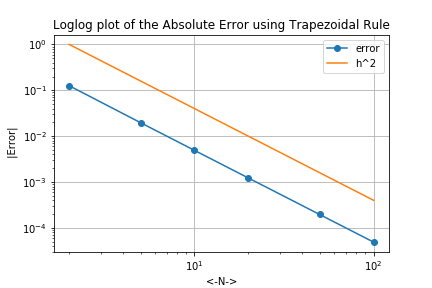
\includegraphics[width=10cm]{TR.png}
     \label{fig:Dendrogram for the problem 3(c)}
     %\end{subfigure}
     \caption{Loglog plot of error using Trapezoidal Rule}
\end{figure}
\begin{figure}[H]  
     \centering
     %\begin{subfigure}[b]{0.3\textwidth}
         %\centering
    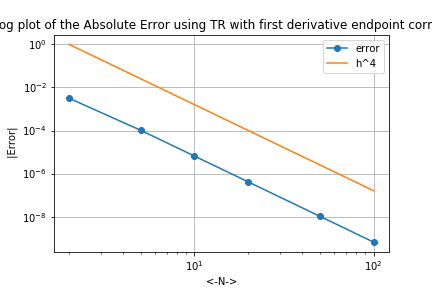
\includegraphics[width=10cm]{TR_1.png}
     \label{fig:Dendrogram for the problem 3(c)}
     %\end{subfigure}
     \caption{Loglog plot of error using Trapezoidal Rule with end corrections using just the first derivative}
\end{figure}
\begin{figure}[H]  
     \centering
     %\begin{subfigure}[b]{0.3\textwidth}
         %\centering
    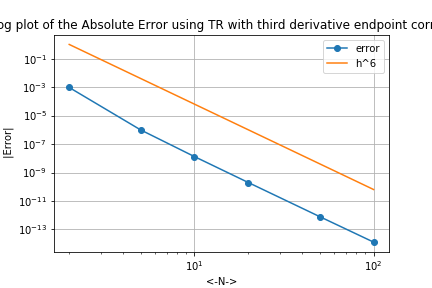
\includegraphics[width=10cm]{TR_3.png}
     \label{fig:Dendrogram for the problem 3(c)}
     %\end{subfigure}
     \caption{Loglog plot of error using Trapezoidal Rule with end corrections using the first derivative and the third derivatives}
\end{figure}
\begin{figure}[H]  
     \centering
     %\begin{subfigure}[b]{0.3\textwidth}
         %\centering
    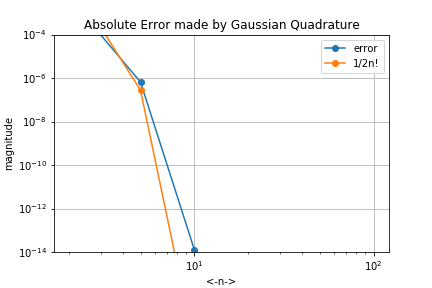
\includegraphics[width=10cm]{Gauss_Quad.png}
     \label{fig:Dendrogram for the problem 3(c)}
     %\end{subfigure}
     \caption{Loglog plot of error using Gauss Legendre Quadrature}
\end{figure}
\begin{figure}[H]  
     \centering
     %\begin{subfigure}[b]{0.3\textwidth}
         %\centering
    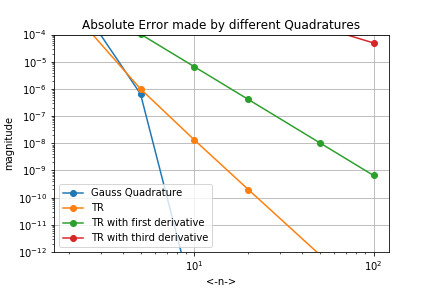
\includegraphics[width=10cm]{Quad.png}
     \label{fig:Dendrogram for the problem 3(c)}
     %\end{subfigure}
     \caption{Loglog plot of error using the different quadratures}
\end{figure}
\textbf{Observations}
\begin{itemize}
    \item As we'd expect, the last method is the best, while plain Trapezoidal Rule is the worst.
    \item We see that the rate of decay of the absolute error follow the same trends derived above.
    \item Thus we can conclude that the four methods do a good job at estimating the given integral even for moderately small values of N.
\end{itemize}
\end{solution}
\question [8] Evaluate I = $\mathlarger{\mathlarger{\int}}_{0}^1 \frac{e^{-x}}{\sqrt{x}} dx$ by subdividing the domain into N $\in  \{5, 10, 20, 50, 100, 200, 500, 1000\} $ panels.
\begin{description}
    \item[(a)] Using a rectangular rule
    \item[(b)]  Make a change of variables x = $t^2$ and use rectangular rule on new variable.
\end{description}
\begin{itemize}
    \item  Plot the decay of the absolute error using the above two methods.
    \item You may obtain the exact value of the integral upto 20 digits using wolframalpha.
    \item Compare the two methods above in terms of accuracy and cost.
    \item Explain the difference in solution, if any.
    \item Make sure the figure has a legend and the axes are clearly marked.
    \item Ensure that the font size for title, axes, legend are readable.
    \item Submit the plots obtained, entire code and the write-up.
\end{itemize}
\begin{solution}
\\
\textbf{True value of the integral:}\\
We obtain the true value of the integral from wolfram alpha and it turns out to be approximately 1.4936482656248540508.\\
\textbf{Integral using substitution}\\
On making the variable change x = $t^2$,dx = 2tdt and the limits remain the same.\\
Thus the integral becomes,
\begin{align*}
    \int_{0}^{1} \frac{e^{-x}}{\sqrt{x}} dx &= \int_{0}^{1} \frac{e^{-t^2}}{t} 2t dt \\
    &\Rightarrow
    \int_{0}^{1} 2e^{-t^2} dt
\end{align*}
\textbf{Rectangular Rule:}\\
Rectangular rule is given as follows:
\begin{align}
    \mathlarger{\mathlarger{\int}}_a^b f(x) dx &= h \cdot \left(\overset{N}{\underset{i=0}{\sum}} f(x_i)\right) + \mathcal{O}\left(h^2\right)
 \end{align}
 for a grid spacing of h and N panels.
 Therefore, applying the rectangular rule on the two integrals, we get the following equations
 \begin{align*}
     \int_{0}^{1} \frac{e^{-x}}{\sqrt{x}} dx &\approx h \cdot \left(\overset{N}{\underset{i=0}{\sum}} \frac{e^{-x_i}}{\sqrt{x_i}}\right)\\
     \int_{0}^{1} 2e^{-t^2} dt &\approx  h \cdot \left(\overset{N}{\underset{i=0}{\sum}} 2e^{-x_i^2} \right)
 \end{align*}
 Using these equations and plotting the error for the given number of panels we obtain the below figure
 \begin{figure}[H]  
     \centering
     %\begin{subfigure}[b]{0.3\textwidth}
         %\centering
    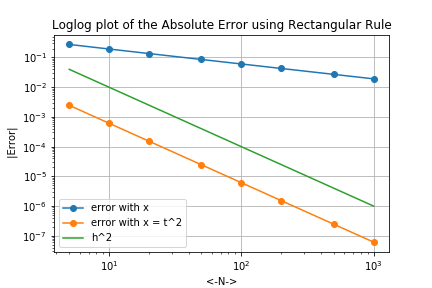
\includegraphics[width=8cm]{Q7.png}
     \label{fig:Dendrogram for the problem 3(c)}
     %\end{subfigure}
     \caption{Plot of the error}
\end{figure}
\textbf{Observations}
\begin{itemize}
    \item As far as computational cost is concerned, we make the same number of function evaluations in both cases. However, as we make an additional division and a square root computation in the first case, we expect it to be more expensive computationally to evaluate the integral in that manner when compared to the substitution case.
    \item The above intuition is substantiated by checking the running time of both the methods for 10000 panels as shown below.
    \begin{verbatim}
Time taken without substitution = 0.011966943740844727
Time taken with substitution = 0.010973453521728516
    \end{verbatim}
    \item As far as the accuracy is concerned, we again see that the substitution case outshines the case without substitution.Moreover, we observe that the case without substitution doesn't even follow the error trends of Rectangular Rule!
    \item Our assumption of using taylor series to derive the Rectangular Rule might not be strictly valid at the endpoints as the function and it's derivative are unbounded at the endpoints.
    \item The variable change draws a parallel to the runge phenomenon, where the runge function was suddenly approximated well as we made the change from uniform nodes. Likewise, the variable change appropriately generates a new series of nodes which turn out to be better for the approximation.
\end{itemize}

\end{solution}
\question [20] Consider the motion of a simple pendulum
\begin{figure}[H]  
     \centering
     %\begin{subfigure}[b]{0.3\textwidth}
         %\centering
    \includegraphics[width=10cm]{NMSC_endsem_1.png}
     \label{fig:Dendrogram for the problem 3(c)}
     %\end{subfigure}
     \caption{Simple Pendulum}
\end{figure}
The restoring force is mg $\sin{\theta}$ and hence the governing equation is
\begin{align*}
    mL \frac{d^2 \theta}{dt^2} + mg\sin{\theta} = 0
\end{align*}
Let the length of the string be g. Hence, the governing equation simplifies to
\begin{align*}
    \frac{d^2 \theta}{dt^2} + \sin{\theta} = 0
\end{align*}
At the initial time, the pendulum is pulled to an angle of $\theta = 30^{\circ}$ = $\frac{\pi}{6}$ before being let loose without any
velocity imparted. Write a code to solve for the motion of the pendulum till t = 100 seconds using
\begin{description}
    \item[(a)] Forward Euler
    \item[(b)] Backward Euler
    \item[(c)] Trapezoidal Rule
\end{description}
\begin{itemize}
    \item Recall that you need to need to reformulate the second order differential equation as a system of first order differential equation.
    \item  Vary your time step $\delta$ t in $\{0.01, 0.02, 0.05, 0.1, 0.2, 0.5, 1, 2, 5, 10, 20\}$.
    \item For each $\delta$ t plot the solution obtained by the three methods on a separate figure till the final time of 100.
    \item Discuss the stability of the schemes. From your plots, at what $\delta $ t do these schemes become unstable (if at all they become unstable)?
    \item Analyse the stability of the three numerical methods to solve the differential equation by approximating $\sin{(\theta)}$ to be $\theta$.
    \item  Make sure each figure has a legend and the axes are clearly marked.
    \item Ensure that the font size for title, axes, legend are readable.
    \item Submit the plots obtained, entire code and the write-up.
\end{itemize}
\begin{solution}
\\
Note: The plots for this question are submitted with the report as they are too many in number and will clutter the report.\\
\textbf{Coupled differential equations}\\
In order to solve this second order ODE we try coupling it into two first order ODEs in the form below.
\begin{align}
    &u^{'} = v\\
    &v^{'} = -\sin{(u)}
\end{align}
where u = $\theta$ and v = $\theta^{'}$.\\
We have the initial values for both of the coupled ODEs.\\
\begin{align}
    &u(0) = \frac{\pi}{6}\\
    &v(0) = 0
\end{align}
\\
\textbf{The different schemes:}\\
We write the different schemes for a time step of dt.\\
\textbf{Forward Euler:}\\
Using the above logic, we have the following forward euler scheme,
\begin{align}
    &\theta^{'}_e[i] = \theta^{'}_e[i-1] - dt(\sin{(\theta_e[i-1])})\\
    &\theta_e[i]      = \theta_e[i-1] + dt(t\theta^{'}_e[i-1])
\end{align}
\textbf{Backward Euler:}\\
To find the backward euler scheme,we consider the first order taylor series approximation of $\sin{(\theta_i[i])}$ and try expressing it in terms of $\theta_i[i-1]$.\\
Thus, as iteration i represents the time t during the iteration i, we write,
\begin{align*}
   \sin{(\theta_i[t])} &\approx \sin{(\theta_i[t-1 + dt])}\\
   &\Rightarrow
   \sin{(\theta_i[t-1])} + dt\cdot\cos{(\theta_i[t-1])}
\end{align*}
Thus, employing this, we have the following backward euler scheme,
\begin{align}
    &\theta^{'}_i[i] = \theta^{'}_i[i-1] - dt(\sin{(\theta_i[i-1])}+dt(\cos{(\theta_i[i-1])}))\\
    &\theta_i[i]      = (\theta_i[i-1] + dt(\theta^{'}_i[i]))
\end{align}
\textbf{Trapezoidal Rule}\\
We employ the same technique employed in the previous case and obtain the following scheme.
\begin{align}
    &\theta^{'}_t[i] = \theta^{'}_t[i-1] - (\frac{dt}{2})(2\sin{(\theta_t[i-1])}+dt(\cos{(\theta_t[i-1])}))\\
    &\theta_t[i] = \theta_t[i-1] + (\frac{dt}{2})(\theta^{'}_t[i]+\theta^{'}_t[i-1])
\end{align}
\\
\textbf{All the schemes with approximation:}\\
Now with the approximation of $\sin{(\theta)} \approx \theta$, the coupled differential equations become,
\begin{align}
    &u^{'} = v\\
    &v^{'} = -(u)
\end{align}
which is similar to the equation of SHM.\\
Thus the schemes now are,\\
\textbf{Forward Euler:}
\begin{align}
    &\theta^{'}_e[i] = \theta^{'}_e[i-1] - dt(\theta_e[i-1])\\
    &\theta_e[i]      = \theta_e[i-1] + dt(t\theta^{'}_e[i-1])
\end{align}
\textbf{Backward Euler:}
The backward euler scheme becomes,\\
\begin{align*}
    &\theta^{'}_i[i] = \theta^{'}_i[i-1] - dt\cdot\theta_i[i]\\
    &\theta_i[i] = \theta_i[i-1] + dt\theta^{'}_i[i]
\end{align*}
Simplifying the above,we have,
\begin{align*}
    \theta^{'}_i[t] = \theta_i[t-1] - dt\cdot\left(\theta_i[t-1] + dt\theta^{'}_i[t]\right)
\end{align*}
On solving for $\theta^{'}_i[t]$ in the above, we get,
\begin{align}
    \theta^{'}_i[i] &= \frac{\theta^{'}_i[i-1] - dt\theta_i[i-1]}{1+(dt)^{2}}
\end{align}
Thus, the backward euler recurrence is,
\begin{align}
    &\theta^{'}_i[i] = \frac{\theta^{'}_i[i-1] - dt\theta_i[i-1]}{1+(dt)^{2}}\\
    &\theta_i[i] = \theta_i[i-1] + dt\theta^{'}_i[i]
\end{align}
\textbf{Trapezoidal Rule:}\\
Similarly for trapezoidal rule, we'll have
\begin{align}
    &\theta^{'}_t[i] = \frac{((1-\frac{(dt)^2}{4})\theta^{'}_t[i-1] - (dt)(\theta_t[i-1]))}{(1 + \frac{(dt)^2}{4})}\\
    &\theta_t[i] = \theta_t[i-1] + (\frac{dt}{2})(\theta^{'}_t[i]+\theta^{'}_t[i-1])
\end{align}
\\
\textbf{Observations}
\begin{itemize}
    \item We see that the backward euler scheme retains the characteristics of the original solution the longest.
    \item The backward euler scheme approximately becomes unstable beyond dt = 1 when there is no approximation of $\sin{(\theta)}$.
    \item The other two schemes become unstable relatively faster at about dt = 0.1 in the absence of approximation of $\sin{(\theta)}$.
    \item That said, for smaller dt, trapezoidal rule deviates much lesser than the forward euler. However for larger dt the deviation is almost the same.
    \item When the approximation is made, we see that the original function plot and approximate function plot exhibit very similar behaviour for the smallest values of dt.
    \item We see that this time however, both the implicit schemes are stable throughout while only the forward euler scheme becomes unstable.
    \item The trapezoidal scheme gives almost the same result that the backward euler scheme gave earlier.
\end{itemize}
\end{solution}
\end{questions}
\end{document}
